\newpage
\chapter[Experimentos e Análise dos Resultados]{Experimentos e Análise dos Resultados}
\label{experimentos}

Como já especificado em capítulos anteriores, este trabalho de dispõe a apresentar um Framework de 
 controle para sistemas discretos de forma a utilizar os principais ganhos do protocolo \ac{MQTT} para propor soluções mais 
 simples do que as amplamente utilizadas em processos industriais para problemas como gerenciamento da rede, custo dos 
 equipamentos utilizados e entre outros. Neste sentido, o principal teste realizado foram a realização de duas provas de
 conceito simulando sistemas amplamente presentes no âmbito industrial para se observar o comportamento do modelo 
 proposto, além disso, a partir das simulações foram encontradas algumas questões para as quais foram propostos testes 
 especiais assim como descrito a seguir.

\section{Método para a Avaliação}
\label{metodo}

O método utilizado para avaliar a funcionalidade do sistema proposto foi a implementação direta de duas provas de 
conceitos utilizando o material do laboratório de ensino de Mecatrônica, isto é, a montagem de um circuito Pneumático 
(primeiramente, mas posteriormente foram feitos testes também com sistemas hidráulicos) para controle de um ou mais 
cilindros utilizando o sistema \ac{MQTT} para promover a comunicação em Edge e em nuvem.

\section{Experimentos}

\subsection{Experimento 1 — Controle de 1 cilindro}

\begin{figure}[htb]
    \begin{center}
	    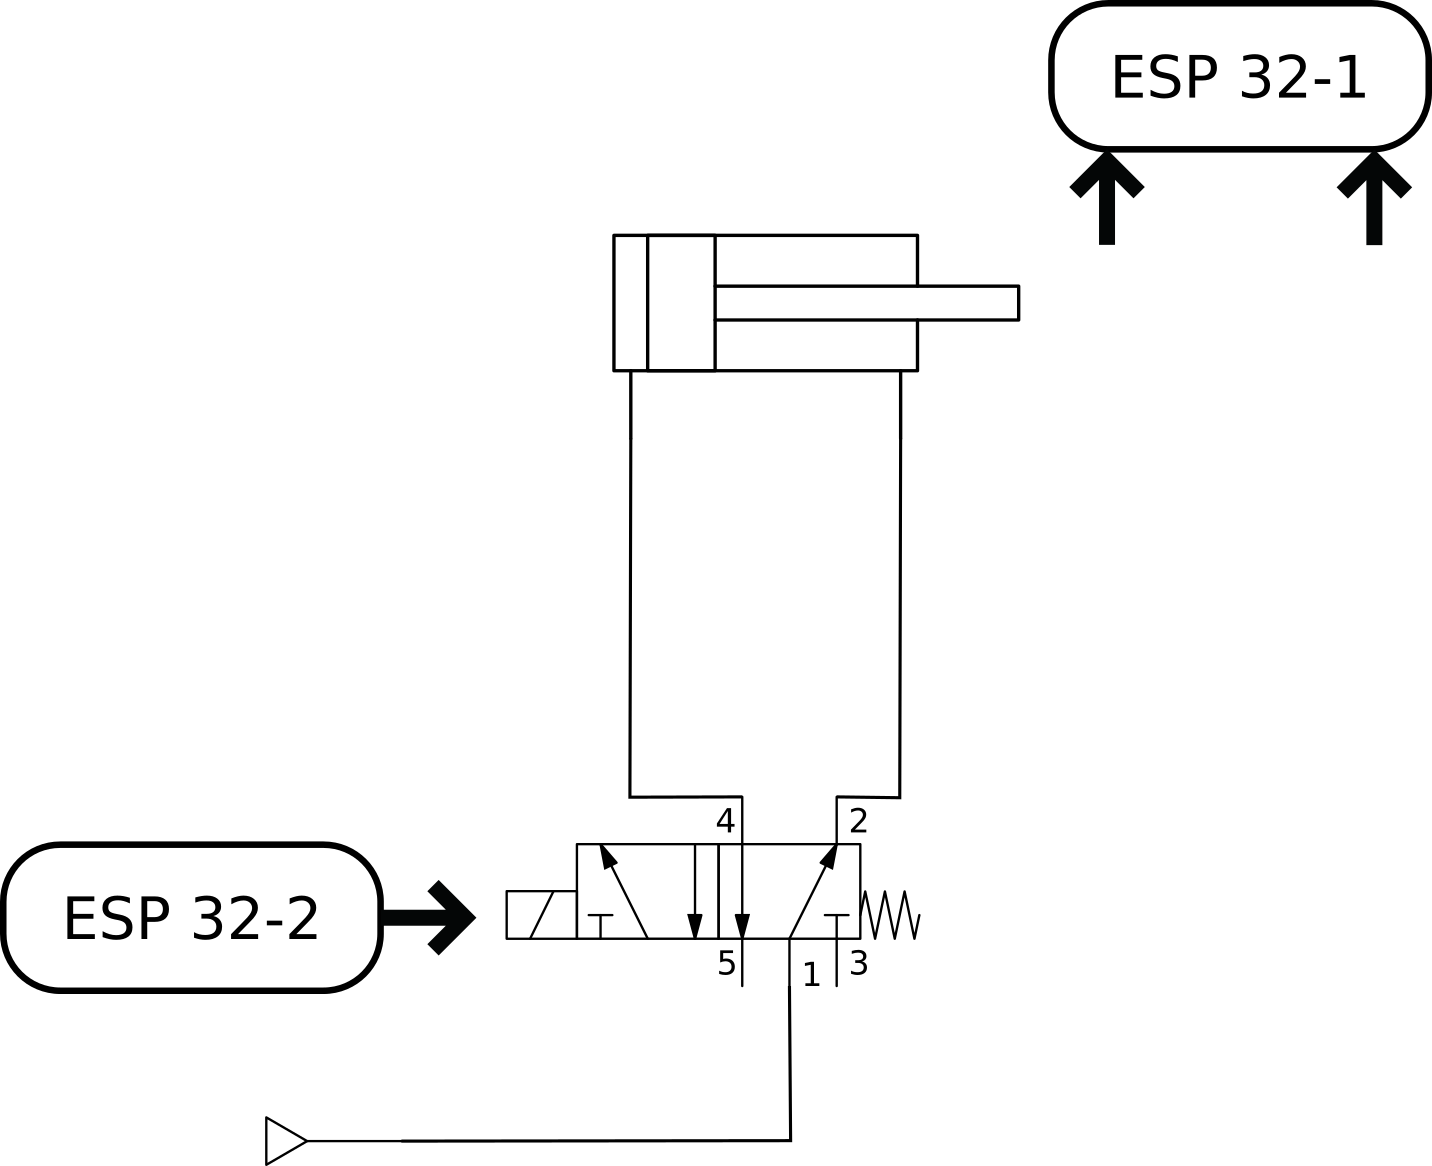
\includegraphics[scale=0.5]{figs/diag_exp1.png}
	\end{center}
	\caption{\label{fig:exp1} Diagrama do primeiro experimento realizado.} 
\end{figure}

O primeiro experimento realizado se dispunha a realizar o controle de apenas um cilindro pneumático de forma que dois
ESP32 foram utilizados no sistema \ac{MQTT} para promover a comunicação, um microcontrolador era responsável por monitorar 
os sensores e disponibilizar seu estado em rede, assim sendo caracterizado como um publicador; enquanto o outro 
microcontrolador era responsável por controlar o estado do cilindro utilizando as informações disponibilizadas pelos 
sensores assim, assim sendo caracterizado como um subscritor. Na \autoref{fig:exp1} existe um diagrama da montagem 
realizada. Neste Exemplo, foram utilizados tanto a implementação local do Broker Eclipse Mosquitto\textregistered~quanto 
o disponibilizado pela AWS\textregistered~, AWS Iot Core. Vale ressaltar que no caso do Broker via AWS foi necessário a 
implementação de Segurança \ac{TLS} e dos Certificados x.509 gerados diretamente na plataforma para a utilização do Broker
\footnote{O caminho para conexão de novos dispositivos pode ser facilmente encontrado no caminho: 
AWS Iot > Connect > Connect one device}, 
desta forma, seguindo o passo a passo descrito na própria plataforma foram geradas a Política e o Certificado de cada ESP
sendo de forma que cada um possui um Endpoint dedicado para conexão, ambos capazes de ler e publicar no tópico "lem/valve"
a \autoref{fig:cert1} mostra a estrutura característica utilizada para cadastro dos itens na AWS. No apendice \autoref{ape:exp1} 
estão disponibilizados os trechos do código responsáveis especificadamente pela transmissão dos dados via \ac{MQTT}, porém
caso queira consultar os codigos completos de cada aplicação eles estão disponíveis e documentados repositório no 
Github\textregistered~ do Laboratório de Planejamento Automático de Manufatura \ac{MAPL} \cite{mapl-repo}.

\begin{figure}[htb]
    \begin{center}
	    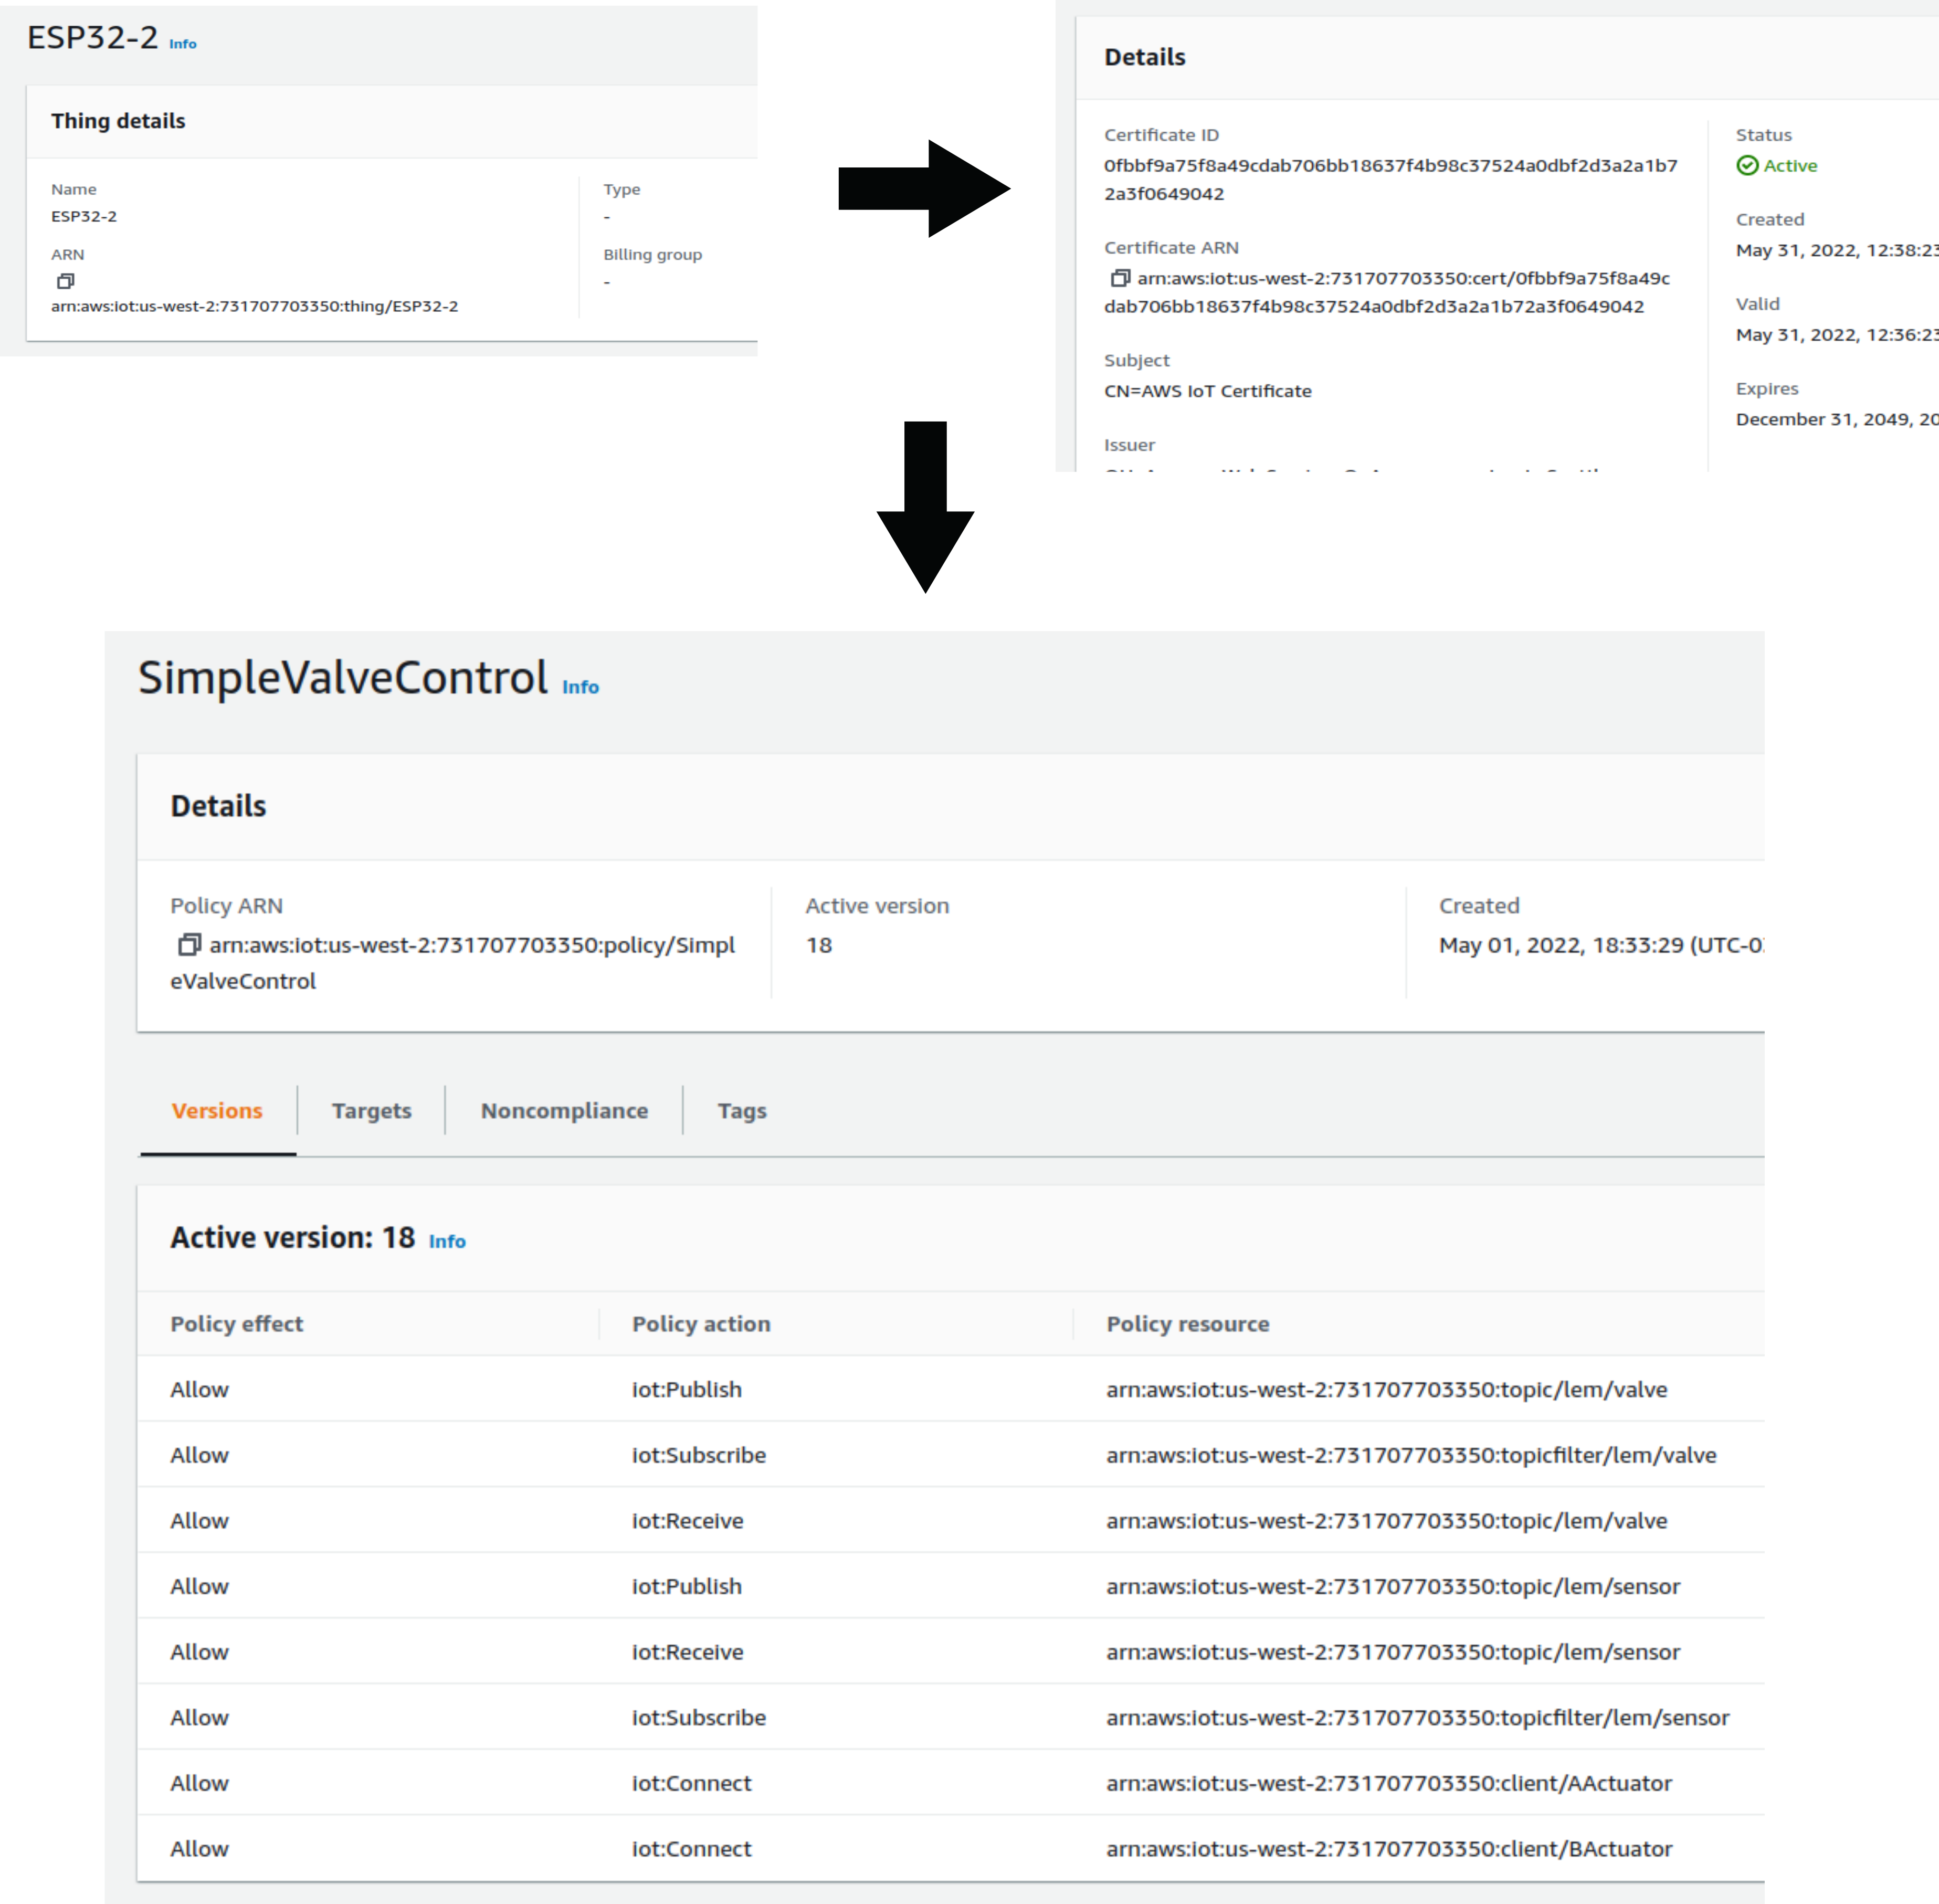
\includegraphics[scale=0.5]{figs/cert_flow.png}
	\end{center}
	\caption{\label{fig:cert1} Estrutura de permissões .} 
\end{figure}


\subsection{Experimento 2 — Controle de 2 cilindros}


\begin{figure}[htb]
    \begin{center}
	    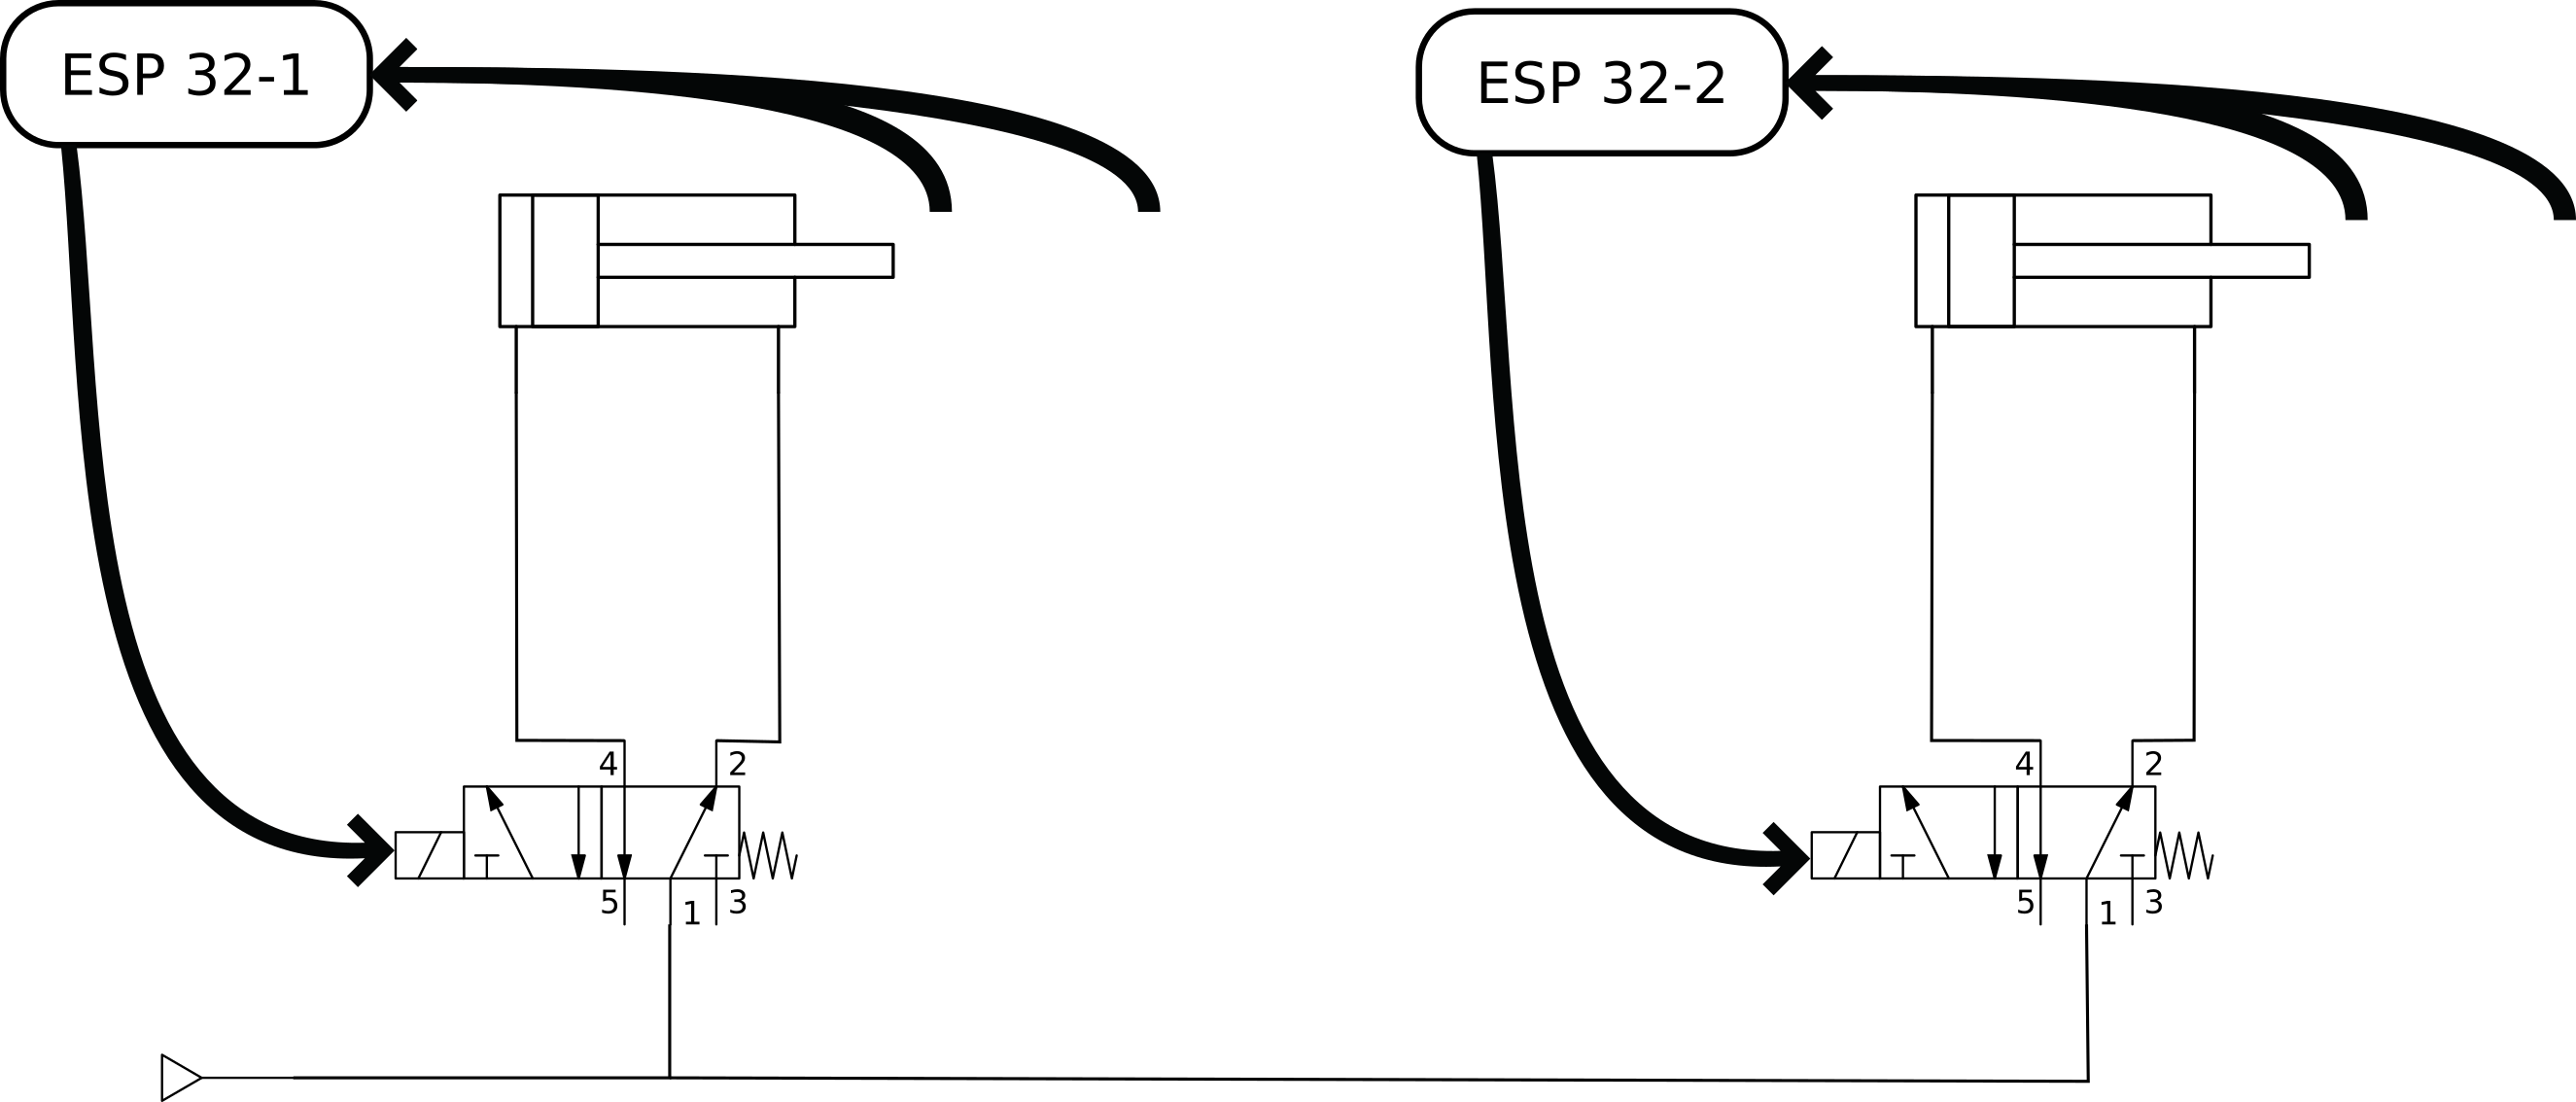
\includegraphics[scale=0.5]{figs/diag_exp2.png}
	\end{center}
	\caption{\label{fig:exp2} Diagrama do segundo experimento realizado.} 
\end{figure}

Já no segundo Experimento, foi utilizada uma montagem onde cada Esp-32 era responsável por um cilindro, isto é, 
controlando tanto suas entradas como suas saídas, assim cada cilindro é, ao mesmo tempo, um publicador e um subscritor.
Na \autoref{fig:exp2} existe um diagrama da montagem realizada. Neste experimento não foram utilizados os recursos da AWS,
em vez disso, agora que já tínhamos testado a comunicação
pela rede deles, neste segundo momento optou-se pelos serviços gratuitos disponibilizados pelo site shiftr.io já que o foco 
não era os elementos de segurança da rede em si, implementação do \ac{SSL} ou geração das permisões. A essa altura o grande
objetivo era a inclusão de um terceiro elemento na rede responsável por duas coisas: funcionar como um servidor de lógica,
ou seja, um item externo que relaciona as saídas dos sensores às entradas dos atuadores e também de um servidor \ac{MQTT} local
que fosse capaz de se comunicar de forma \textit{full-duplex} com o servidor em nuvem, permitindo que o sistema fosse acessado 
remotamente, mas sem deixá-lo totalmente dependente da nuvem, de forma que o mesmo continua funcionando em casos em que 
a comunicação entre a rede local e a Internet é perdida. O arquivo de configuração do \textit{Broker} local pode ser consultado
no \autoref{ape:moss}.

\begin{figure}[htb]
    \begin{center}
	    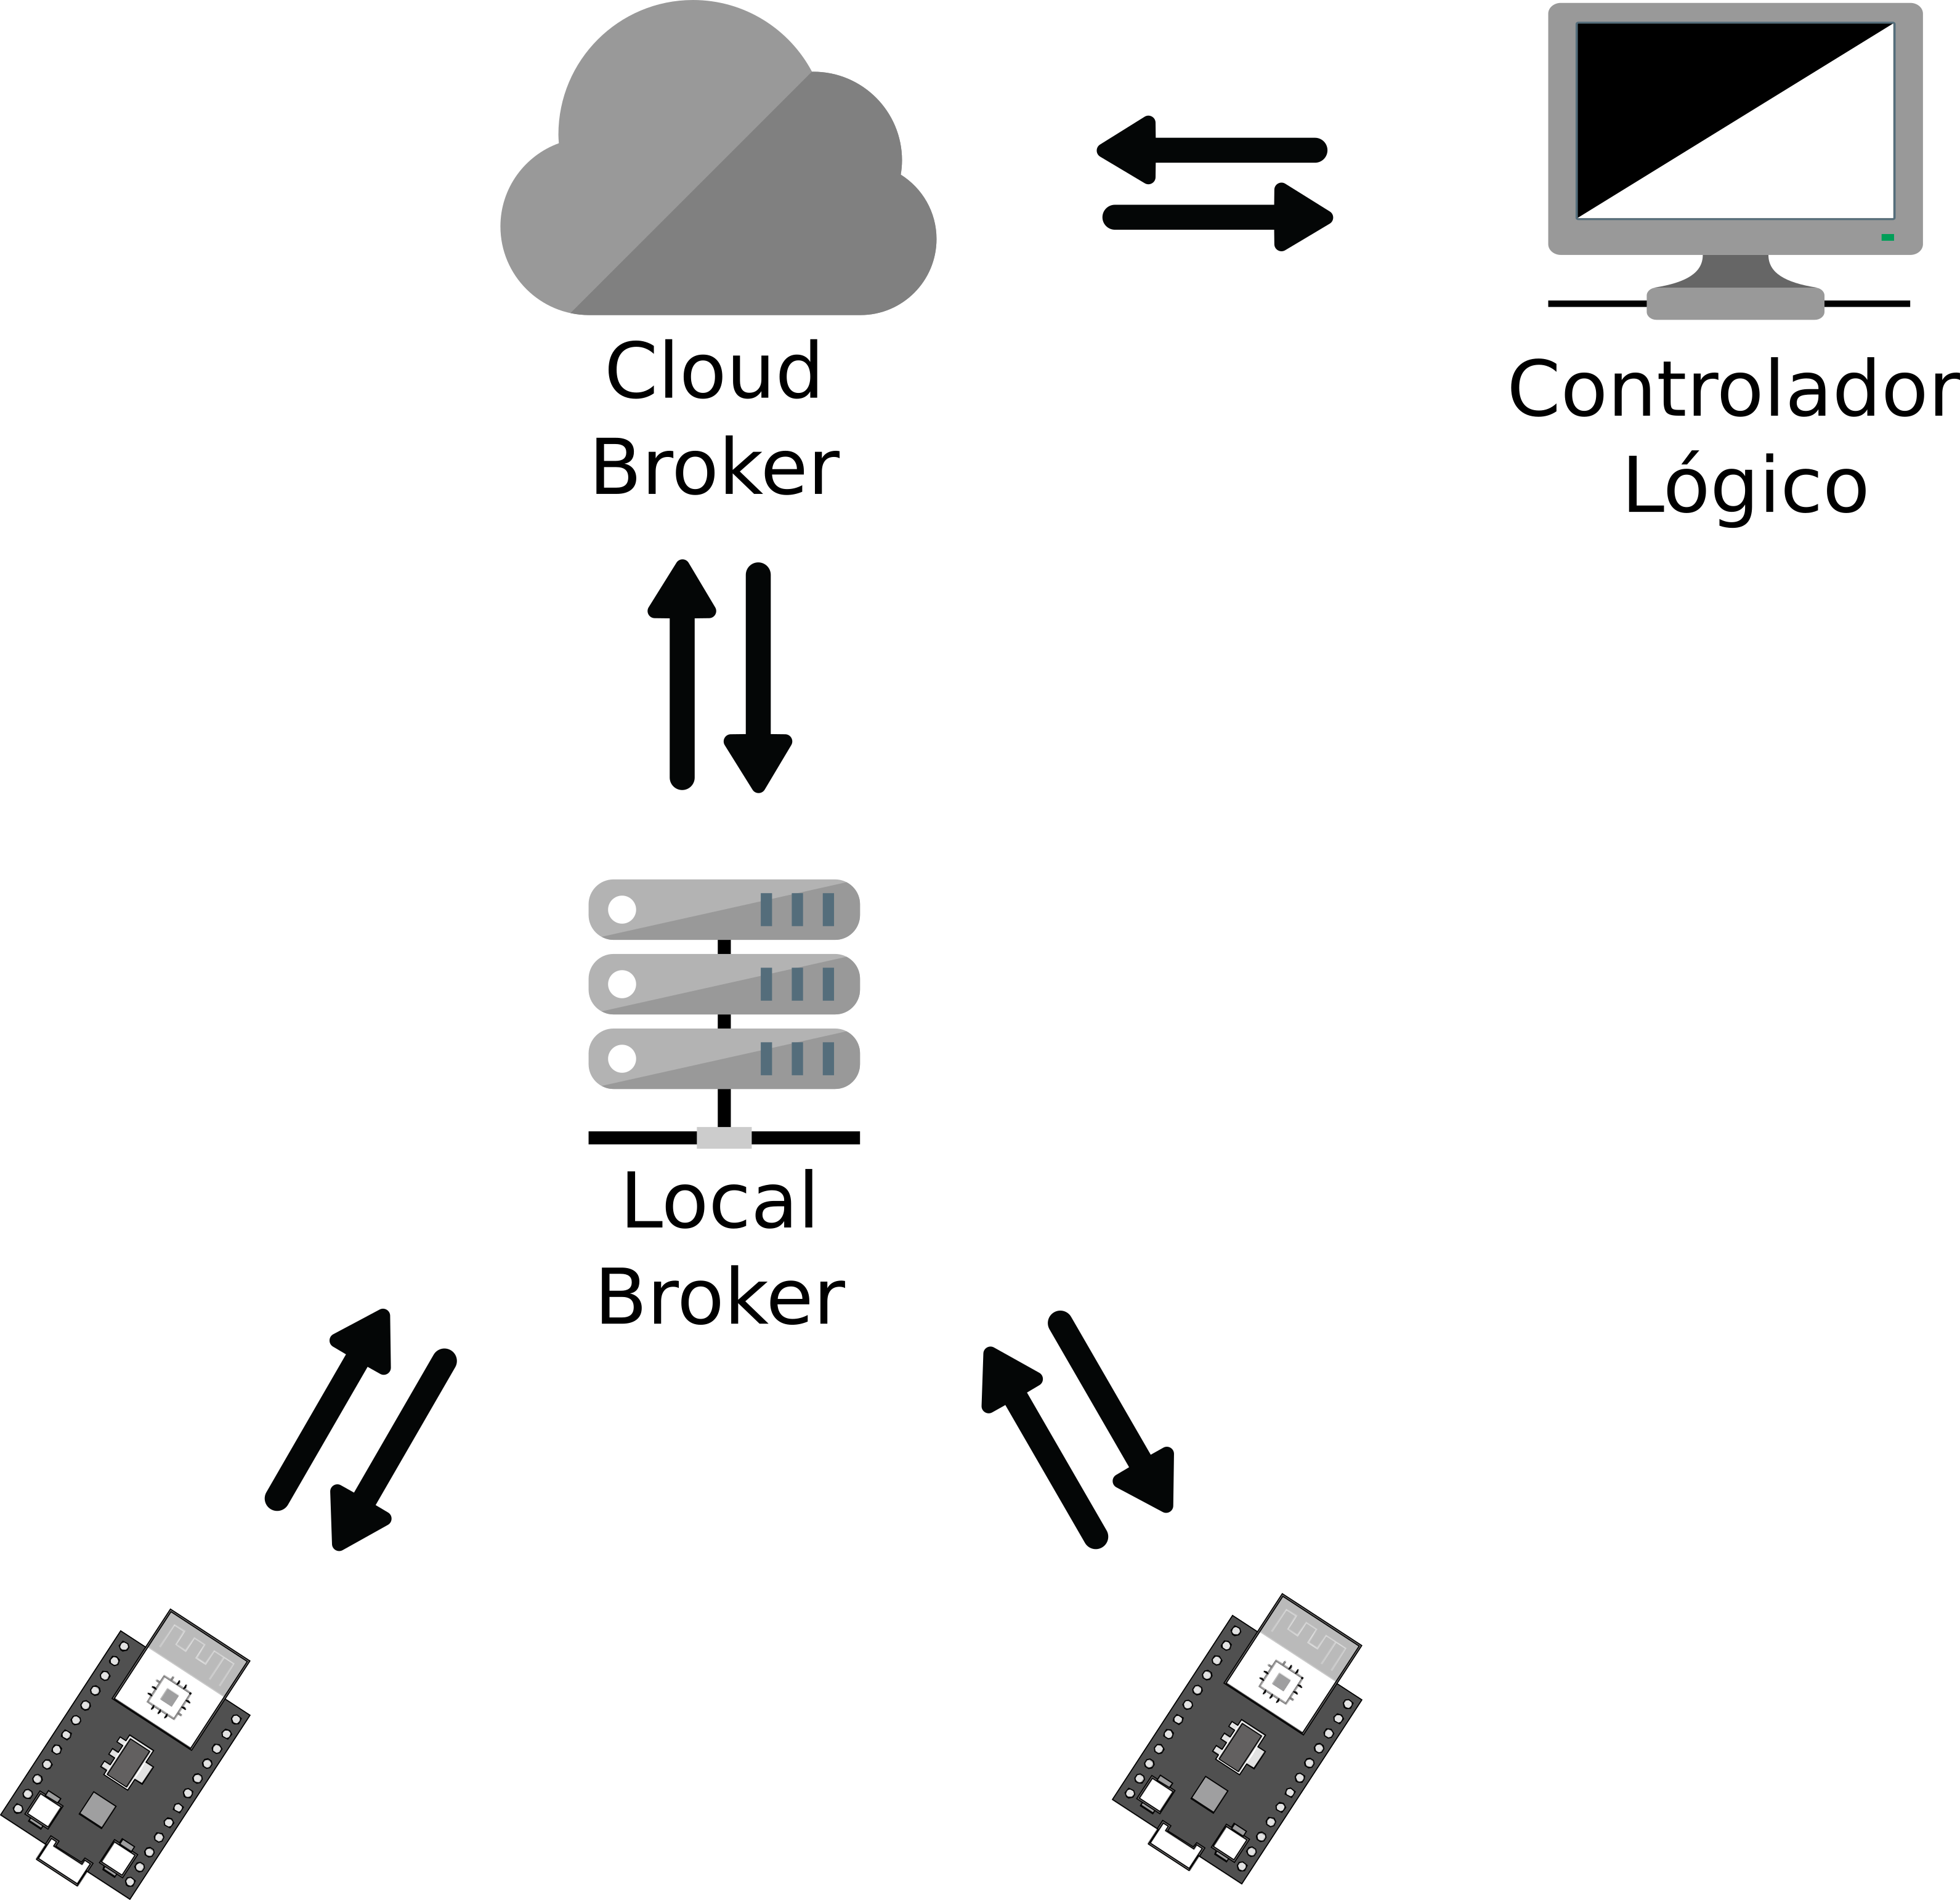
\includegraphics[width=200pt]{figs/diag_conn.png}
	\end{center}
	\caption{\label{fig:exp2} Diagrama da comunicação entre o Broker local e em nuvem.} 
\end{figure}


Como elemento extra foi utilizado a título de exemplo um Raspberry Pi 4; no qual, beneficiando-se do isolamento de processos 
característico de sistemas operacionais, era possível a implementação simultânea do broker \ac{MQTT} Mosquitto e de um script 
python para controle do sistema. Assim, para a parte de lógica foi utilizada a biblioteca própria para comunicação com 
servers \ac{MQTT} paho, pois dada a praticidade dos scripts python ficava bem simples a aplicação da lógica e a implementação 
de possíveis modificações já com o sistema funcionando. Por fim, na implementação do Broker mosquitto foi utilizada uma 
função chamada \ac{MQTT} Bridge\cite{mosq-doc} configurada de forma que todos os tópicos utilizados no sistema estão sendo 
replicados nos dois Brokers assim garantindo que uma queda na Internet não quebrará todo o sistema, além de possibilitar
que sejam colocados lógicas de segurança em Edge para casos onde uma parada abrupta geraria sérios problemas.

\section{Avaliação dos Resultados}
\label{avaliacao}

\begin{figure}[htb]
    \begin{center}
        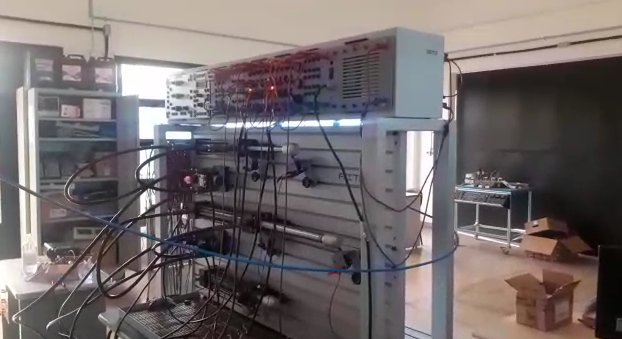
\includegraphics[scale=0.5]{figs/exp_h.png}
    \end{center}
    \caption{\label{fig:exp2} Montagem realizada na bancada hidráulica.} 
\end{figure}

\begin{figure}[htb]
    \begin{center}
	    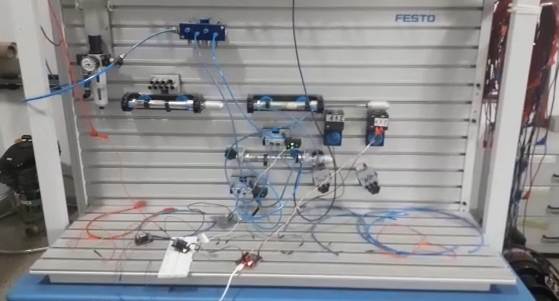
\includegraphics[scale=0.5]{figs/exp_p.png}
	\end{center}
	\caption{\label{fig:exp2} Montagem realizada na bancada pneumática.} 
\end{figure}


Após a implementação em bancada do sistema, obteve-se grande sucesso com a comunicação e com o funcionamento do sistema como um todo,
em ambas as montagens. Porém, foram encontradas alguns problemas na transmissão das informações que, embora não sejam
capazes de inviabilizar o sistema conforme os objetivos preestabelecidos para o estudo atual, são possíveis objetos de 
estudo para trabalhos posteriores, sendo eles principalmente o aumento da lentidão na troca de informações dependendo da 
Nuvem utilizada, o que não era perceptível no primeiro teste, na bancada hidráulica; mas acabou ficando evidente nos testes
utilizando o circuito pneumático e a inclusão de ruído proveniente dos sensores utilizados na montagem
também a depender do atuador e dos sensores de contato utilizados. Vale ressaltar, ainda, que a velocidade na transmissão
de mensagens sofria grandes variações de acordo com o \textit{Broker} utilizado, sendo praticamente instantânea em aplicações com
\textit{Broker} local, tendo pequeno atraso quando instanciado utilizando a nuvem AWS, e maior atraso quando utilizada a
nuvem disponibilizada pelo \textit{shiftr.io}~\textregistered.